% Centri — introductory overview talk for a general audience (2026-07-27)
%
% NOT a weekly deck. Different job, different treatment: this is a visual aid for a SPOKEN talk to
% people who are not physicists and have not seen the project, so the slides are lighter than the
% weekly decks (which follow rule #5 in CLAUDE.md — read cold, no narration — because they are
% read, not presented). Each slide still closes on a one-line takeaway, so it is not meaningless
% without the talk. Overview style: breadth over depth, a picture on nearly every slide.
%
% PACING. Twelve content slides is about 14–15 minutes at a comfortable pace.
% To bring it to 10 minutes, drop these three and the story still holds:
%     "How it works, end to end" · "What it is built on" · "Why these teaching choices"
% Everything else is the narrative spine.
%
% Compile: pdflatex -interaction=nonstopmode centri-talk-intro-2026-07-27.tex  (run twice)
\documentclass[aspectratio=169,11pt]{beamer}
\usetheme{metropolis}
\metroset{sectionpage=none, subsectionpage=none, numbering=fraction, progressbar=frametitle}

\usepackage{booktabs}
\usepackage{xcolor}
\usepackage{colortbl}
\usepackage{graphicx}
\graphicspath{{figs/}}
\usepackage[most]{tcolorbox}
\usepackage{tikz}
\usetikzlibrary{arrows.meta, positioning, shapes.geometric}

% ---- palette (shared with the other Centri decks) ------------------------
\definecolor{cMeas}{HTML}{1F6FB2}
\definecolor{cPed}{HTML}{B5651D}
\definecolor{cApp}{HTML}{2E7D32}
\definecolor{cInfra}{HTML}{5E35B1}
\definecolor{cAccent}{HTML}{C62828}
\definecolor{cGrey}{HTML}{616161}
\definecolor{cBasic}{HTML}{2E7D32}
\definecolor{cInter}{HTML}{1F6FB2}
\definecolor{cAdv}{HTML}{5E35B1}
\setbeamercolor{frametitle}{bg=cApp}
\setbeamercolor{progress bar}{fg=cAccent}

\newcommand{\takeaway}[1]{\vfill{\small\itshape\color{cGrey}#1\par}}

\title{Physics Lessons From a Phone Video}
\subtitle{Point a camera at something spinning, and get a worksheet back --- an overview}
\author{Damar Albaribin}
\institute{MSc Thesis --- advisor: Prof.\ Wu-Yuin Hwang}
\date{2026-07-27}

\begin{document}
\maketitle

% =========================================================================
\begin{frame}{Where this starts}
\begin{columns}[T]
\begin{column}{0.56\textwidth}
\vspace{4pt}
\small
Students meet circular motion as a \textbf{diagram in a textbook} --- a perfect circle, a tidy
arrow, numbers chosen to divide neatly.
\vspace{8pt}

Doing it for real needs \textbf{lab equipment} most classrooms do not have.
\vspace{8pt}

But everybody has a \textbf{phone}. And things that go round are everywhere: a ceiling fan, a
turntable, a playground wheel.
\vspace{10pt}

{\color{cApp}\textbf{So: can a computer watch fifteen seconds of ordinary video and write the
physics lesson from what it sees?}}
\end{column}
\begin{column}{0.42\textwidth}
\centering
\includegraphics[height=0.62\textheight]{talk-wheel-plain.jpg}\\[2pt]
{\scriptsize\color{cGrey}One of the seven clips: a playground wheel, filmed on a phone.}
\end{column}
\end{columns}
\takeaway{No sensors, no lab kit, no special camera --- just the video.}
\end{frame}

% =========================================================================
\begin{frame}{Everything one clip produces}
\vspace{-3pt}
{\small From a single fifteen-second video, with nobody typing anything in:}
\vspace{1pt}

\begin{center}
\includegraphics[width=\textwidth]{talk-artifacts.png}
\end{center}

{\scriptsize Graphs, marked-up pictures, a video with the physics drawn onto the moving footage, a
measurements table --- and \textbf{six documents}: three levels of worksheet, each with a teacher's
copy.}
\takeaway{Every number on all of these came out of the footage. Nothing was entered by hand.}
\end{frame}

% =========================================================================
\begin{frame}{Seeing the physics on the footage}
\begin{columns}[T]
\begin{column}{0.30\textwidth}
\centering
\includegraphics[height=0.70\textheight]{talk-annot-video.jpg}
\end{column}
\begin{column}{0.68\textwidth}
\vspace{6pt}
\small
The same four things are drawn on the still picture, on the graphs, and onto \textbf{every frame of
the moving video}:
\vspace{8pt}

\begin{tabular}{@{}ll@{}}
{\color{cAccent}$\longleftrightarrow$} & how far out it sits from the centre \\[4pt]
{\color{cMeas}$\longrightarrow$} & how fast it travels along the circle \\[4pt]
{\color{cPed}$\curvearrowright$} & how fast it sweeps round the centre \\[4pt]
{\color{cAdv}$\longrightarrow$} & the inward pull that keeps it on the circle \\
\end{tabular}
\vspace{10pt}

For the beginner's worksheet the same four arrows are kept, but every label is written
\textbf{in words} instead of symbols --- the picture is where a beginner does most of the work, so
it is the last thing that should be stripped down.
\end{column}
\end{columns}
\takeaway{The learner sees the physics on the object they actually filmed, not on an idealised
drawing of it.}
\end{frame}

% =========================================================================
\begin{frame}{Why it isn't easy}
\begin{columns}[T]
\begin{column}{0.40\textwidth}
\vspace{2pt}
\small
A sensor \emph{tells} you how fast something spins. A video tells you nothing --- it is only
coloured dots.
\vspace{8pt}

Every number has to be worked out from where the object appears, frame by frame. That can go wrong
while looking completely convincing.
\vspace{8pt}

{\color{cAccent}\textbf{On the left, the spot being followed has drifted off the handle
entirely.}} The worksheet built from it would still look perfect.
\end{column}
\begin{column}{0.29\textwidth}
\centering
\includegraphics[width=\textwidth]{wheel_naive_crop.png}\\[3pt]
{\scriptsize\textbf{\color{cAccent}Confidently wrong}}
\end{column}
\begin{column}{0.29\textwidth}
\centering
\includegraphics[width=\textwidth]{wheel_corrected_crop.png}\\[3pt]
{\scriptsize\textbf{\color{cApp}Right}}
\end{column}
\end{columns}
\takeaway{A wrong measurement produces an equally beautiful worksheet. That is the whole problem.}
\end{frame}

% =========================================================================
\begin{frame}{It shows its working}
\begin{columns}[T]
\begin{column}{0.40\textwidth}
\vspace{2pt}
\small
The wheel was filmed slightly from the side, so the handle \emph{appears} to race and stall once
every turn. That is the camera, not the wheel.
\vspace{8pt}

Rather than quietly fixing it, the worksheet draws \textbf{both} lines: what came off the video,
and what it was corrected to.
\vspace{8pt}

{\color{cApp}A student can \emph{see} what was taken out, instead of being told to trust the
answer.}
\end{column}
\begin{column}{0.58\textwidth}
\centering
\vspace{4pt}
\includegraphics[width=\textwidth]{wheel-ac-shipped.png}
\end{column}
\end{columns}
\takeaway{Being honest about a measurement is itself worth teaching --- and it takes real data to
teach it with.}
\end{frame}

% =========================================================================
\begin{frame}{How it works, end to end}
\vspace{2pt}
{\small Nine stages. The two shaded ones are \textbf{checks}: nothing moves past them unexamined.}
\vspace{6pt}

\begin{center}
\resizebox{\textwidth}{!}{%
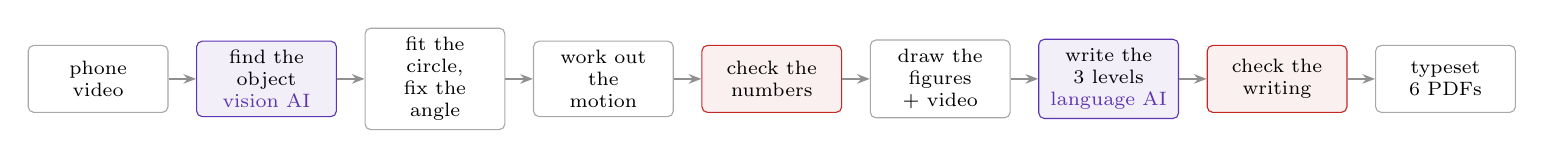
\begin{tikzpicture}[
  node distance=3.5mm,
  box/.style={draw=cGrey!55, rounded corners=2pt, fill=white, align=center,
              font=\scriptsize, inner sep=3.2pt, text width=15.5mm, minimum height=8.5mm},
  chk/.style={box, draw=cAccent, fill=cAccent!7, text=black},
  ai/.style={box, draw=cInfra, fill=cInfra!8},
  arr/.style={-{Stealth[length=1.6mm]}, cGrey!70, thick}]
\node[box] (v) {phone\\video};
\node[ai, right=of v] (t) {find the\\object\\{\scriptsize\color{cInfra}vision AI}};
\node[box, right=of t] (g) {fit the\\circle,\\fix the\\angle};
\node[box, right=of g] (k) {work out\\the\\motion};
\node[chk, right=of k] (c1) {check the\\numbers};
\node[box, right=of c1] (f) {draw the\\figures\\+ video};
\node[ai, right=of f] (w) {write the\\3 levels\\{\scriptsize\color{cInfra}language AI}};
\node[chk, right=of w] (c2) {check the\\writing};
\node[box, right=of c2] (p) {typeset\\6 PDFs};
\foreach \a/\b in {v/t, t/g, g/k, k/c1, c1/f, f/w, w/c2, c2/p} \draw[arr] (\a) -- (\b);
\end{tikzpicture}}
\end{center}
\vspace{6pt}

\begin{columns}[T]
\begin{column}{0.48\textwidth}
{\scriptsize\textbf{\color{cInfra}Only two stages use AI.} One finds the object in the footage; one
writes the prose. Everything between is ordinary arithmetic --- so the same video always gives the
same numbers.}
\end{column}
\begin{column}{0.48\textwidth}
{\scriptsize\textbf{\color{cAccent}The checks are not AI either.} Plain rules: does the arithmetic
add up, does every number appear in the measurements, is the wording right for the level, does the
description match the graph.}
\end{column}
\end{columns}
\takeaway{The AI is asked to do the two things it is good at, and is not trusted with the
arithmetic.}
\end{frame}

% =========================================================================
\begin{frame}{What it is built on}
\vspace{1pt}
\scriptsize
\renewcommand{\arraystretch}{1.32}
\begin{center}
\begin{tabular}{@{}p{3.4cm}p{4.5cm}p{4.6cm}@{}}
\toprule
\rowcolor{cInfra!10}
\textbf{Stage} & \textbf{What does it} & \textbf{Note} \\
\midrule
finding the object & \textbf{SAM3}, a video segmentation model, on a local GPU &
told what to look for in plain words \\
measuring & \textbf{Python}, NumPy, SciPy & no model at all --- same input, same answer \\
figures and the video & \textbf{Matplotlib}, \textbf{OpenCV} & the video is drawn frame by frame \\
writing the worksheets & \textbf{Qwen3.6-35B}, on our own machine & one call per level \\
checking the writing & \textbf{Python}, rule-based & about a hundred checks, no model \\
the documents & \textbf{\LaTeX} & six PDFs per clip \\
running it all & \textbf{FastAPI}, \textbf{Celery}, \textbf{Redis}, \textbf{Docker} & a queue, so a
phone can upload and walk away \\
the phone app & \textbf{Flutter} & record, mark the object, get the worksheets back \\
\bottomrule
\end{tabular}
\end{center}
\takeaway{Everything runs on hardware in the lab --- no cloud service ever sees a student's video.}
\end{frame}

% =========================================================================
\begin{frame}{Three levels, one video}
\vspace{2pt}
\small
The same clip becomes three worksheets, for three readers. They are written from the \emph{same}
measured numbers, so they differ in difficulty without ever disagreeing on fact.
\vspace{6pt}

\renewcommand{\arraystretch}{1.5}
\begin{center}
\begin{tabular}{@{}lp{7.3cm}c@{}}
\toprule
\rowcolor{cApp!12}
\textbf{Level} & \textbf{What the reader is asked to do} & \textbf{ideas at once} \\
\midrule
\textbf{\color{cBasic}Basic} & name what is being measured, and say what each one means --- in
words, with no formulas at all & 5 \\
\textbf{\color{cInter}Intermediate} & read the graph, then meet the equation that says the same
thing, and put this wheel's numbers into it & 19 \\
\textbf{\color{cAdv}Advanced} & compare two moments, compare the parts of the motion, and judge
which claims the video actually supports & 44 \\
\bottomrule
\end{tabular}
\end{center}
\vspace{4pt}

{\scriptsize\color{cGrey}The last column is counted from the finished text --- how many quantities
and links between them the reader has to hold at the same time. It rises on all seven clips, so the
ladder is measured rather than asserted.}
\takeaway{The levels differ in the thinking they ask for, not in how many numbers they contain.}
\end{frame}

% =========================================================================
\begin{frame}{Why these teaching choices}
\vspace{-1pt}
{\scriptsize Nothing in the design is a matter of taste --- each choice comes from a known result
in how people learn.}
\vspace{2pt}

\scriptsize
\renewcommand{\arraystretch}{1.16}
\begin{center}
\begin{tabular}{@{}p{6.1cm}p{6.4cm}@{}}
\toprule
\rowcolor{cPed!12}
\textbf{What the material does} & \textbf{Why} \\
\midrule
three levels, split by how many ideas must be held at once &
cognitive load --- difficulty is how much has to be juggled together \\
each level asks a different \emph{kind} of thinking: name it, apply it, judge it &
Bloom's taxonomy of learning objectives \\
predict what will happen before the measurement is shown &
predict--observe--explain: a guess you committed to is what makes the answer stick \\
first worked example complete, later ones stop halfway &
a full example helps a beginner, and stops helping once the pattern is learned \\
the common wrong answers are asked about directly &
a misconception never voiced is never given up \\
answers only in the teacher's copy &
retrieving an answer teaches more than reading one \\
a last question set somewhere else entirely &
an idea tied to one object has not transferred \\
\bottomrule
\end{tabular}
\end{center}
\takeaway{The physics comes from the video; the shape of the lesson comes from the research on
learning.}
\end{frame}

% =========================================================================
\begin{frame}{Not a page to read}
\vspace{2pt}
\small
Reading about physics is one of the weakest ways to learn it. A worksheet built from a video can do
something a textbook cannot: \textbf{it can stop before the answer.}
\vspace{10pt}

\begin{columns}[T]
\begin{column}{0.31\textwidth}
\textbf{\color{cApp}Predict first.}\\[4pt]
{\small Before any measurement is shown: does it go round faster or slower as the clip goes on?
Commit, then look.}
\end{column}
\begin{column}{0.31\textwidth}
\textbf{\color{cApp}Check before you go on.}\\[4pt]
{\small Each level is three steps, and each step ends with one question you have to be able to
answer.}
\end{column}
\begin{column}{0.31\textwidth}
\textbf{\color{cApp}Meet the traps.}\\[4pt]
{\small The wrong answers most people hold --- said out loud and asked about, rather than left
unmentioned.}
\end{column}
\end{columns}
\vspace{10pt}

{\color{cGrey}\small None of it is guesswork: every question and every answer is computed from the
same measurements, so it is right on every clip.}
\takeaway{The reader is asked to do something roughly every page --- and the answers live in the
teacher's copy.}
\end{frame}

% =========================================================================
\begin{frame}{Where it stands}
\vspace{2pt}
\begin{columns}[T]
\begin{column}{0.48\textwidth}
\textbf{\color{cApp}What is settled}
\vspace{6pt}

{\small
Seven clips --- ceiling fans, turntables, a playground wheel --- carried all the way from video to
finished worksheet.
\vspace{6pt}

Every number checked against the footage it came from, automatically, before anyone reads it:
\textbf{21 of 21} worksheets pass every check.
\vspace{6pt}

A physics teacher read the material, and that review reshaped it --- and turned up a real error in
the physics.}
\end{column}
\begin{column}{0.48\textwidth}
\textbf{\color{cAccent}What is not}
\vspace{6pt}

{\small
Everything measured so far is a property of the \emph{worksheet}: are its numbers right, is it
readable, does it ask enough of the reader.
\vspace{6pt}

\textbf{Nothing yet measures whether anybody learns from it.}
\vspace{6pt}

That is the next study: put it in front of teachers and students, and find out.}
\end{column}
\end{columns}
\takeaway{The measurement problem is largely solved. The teaching question is still open --- and it
is the more interesting one.}
\end{frame}

% =========================================================================
\begin{frame}{In one sentence}
\vspace{12pt}
\begin{tcolorbox}[colback=cApp!6,colframe=cApp,boxsep=4pt,left=10pt,right=10pt,top=8pt,bottom=8pt]
\large A phone video of something spinning becomes physics worksheets at three levels --- with every
number measured from the footage, checked before it ships, and the working shown rather than
asserted.
\end{tcolorbox}
\vspace{14pt}

\centering
{\large\color{cGrey}Thank you --- questions welcome.}
\end{frame}

\end{document}
